\documentclass{../../../ExampleProblem}
\usepackage{../../../mathshortcuts}


\title{Beam Design}
\author{Brian Chevalier}
\subtitle{Beam Design}
\coursenum{CEE421}
\coursetitle{Concrete Design}
\university{gitMechanics}
\date{\today}

% Add to glossary
% Check mathshortcuts.sty for documentation
\glo{Mu}{M_{u}}{Factored ultimate moment in the beam}
\glo{Mn}{M_n}{Nominal moment strength}
\glo{As}{A_s}{Area of tension reinforcing steel}
\glo{bb}{b}{Width of compression zone in a beam}
\glo{dd}{d}{Distance from the extreme fiber in compression}

\glo{rhob}{\rho_b}{The reinforcement ratio of concrete at the balance condition}

\glo{fy}{f_y}{Yield stress of steel}
\glo{fs}{f_s}{Stress of the steel}
\glo{fc}{f'_c}{Yield stress of concrete}
\glo{betao}{\beta_1}{ACI variable}

\glo{ecu}{\varepsilon_{cu}}{Ultimate compressive strain of concrete}
\glo{ey}{\varepsilon_y}{Yield strain of steel}
\glo{es}{\varepsilon_s}{Strain of tension steel}


\begin{document}

\problemstatement
{
	Select the area of steel, $A_s$, cross section width, $b$, and effective depth $d$ for the cross section shown. Satisfy ACI code strength requirements.
}
{
	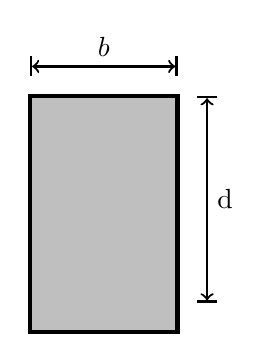
\begin{tikzpicture}[scale=0.75]
		\draw[ultra thick,fill=lightgray] (0,0)rectangle(2.5,4);
		\draw[thick,|<->|] (0,4.5)--node[above]{$b$}(2.5,4.5);
		\draw[thick,|<->|] (3,0.5) --node[right]{d}(3,4);
		\poi{0.5,0.5}
		\poi{1,0.5}
		\poi{1.5,0.5}
		\poi{2,0.5}
	\end{tikzpicture}
}


\section{Solution Strategy}
To solve this problem we must start with the basic design relationship, assume the steel is yielding, estimate the beam weight and perform structural analysis to find the ultimate moment in the beam. Next we must estimate a reinforcement ratio and $bd^2$. We can then select our quantities, find the required area of steel, select the number of standardized bars required, verify that the section is adequate and in tension control.


The diagrams below from left to right are the cross section sketch, strain diagram, stress diagram, and free body diagram. These diagrams will be used to derive the design relationship.

\begin{center}
\begin{tikzpicture}[xscale=1.1]
	%% Cross section
	\draw[ultra thick] (1.5,3) rectangle (0,0);
	
	%% height
	\draw[thick,|<->|] (-0.5,0) -- node[left]{h} (-0.5,3);
	
	%% base
	\draw[thick,|<->|] (0,3.5) -- node[above]{b} (1.5,3.5);
	
	%% depth to steel
	\draw[thick,|<->|] (2,0.5) -- node[right]{d} (2,3);
	
	\draw[dashed, thin] (0,0.5) -- (10,0.5);
	
	\draw[dashed, thin] (-1,0) -- (10,0);
	\draw[dashed, thin] (-1,3) -- (10,3);
	
	%Steel circles
	\draw[ultra thick,fill=white] (0.5,0.5) circle (0.1cm);
	\draw[ultra thick,fill=white] (1,0.5) circle (0.1cm);
	
	%% Strain axis line
	\draw[ultra thick] (4,0) -- (4,3);
	% strain plot and labels
	\draw[thick,|<->|] (2.9,-0.5) -- node[below]{\es$\geq$\ey} (4,-0.5);
	\draw[dashed, thin] (2.9,-0.5) -- (2.9,0.5);
	
	\draw[thick] (2.5,0) -- (5,3);
	\draw[thick,|<->|] (5,3.5) -- node[above]{\ecu} (4,3.5);
	%Neutral axis
	\draw[thin, dashed] (3,1.8) -- (10, 1.8);
	% Depth to neutral axis line
	\draw[thick, |<->|] (3,1.8) -- node[left]{c} (3,3);
	
	\begin{scope}[xshift=-0.5cm]
	%% Stress axis line
	\draw[ultra thick] (7,0) -- (7,3);
	\draw[thick,|<->|] (6,2) -- node[left]{a} (6,3);
	\draw[thin, dashed] (6,2) -- (10,2);
	
	\draw[thick,|<->|] (7,3.5) -- node[above]{0.85\fc} (8,3.5);
	\draw[thick,|<->|] (6,-0.5) -- node[below]{\fs=\fy} (7,-0.5);
	
	%whitney stress block arrows
	\draw[thick,red,->] (8,3) -- (7,3);
	\draw[thick,red,->] (8,2.5) -- (7,2.5);
	\draw[thick,red,->] (8,2) -- (7,2);
	\draw[thick, red] (8,3) -- (8,2);
	
	% Steel stress
	\draw[thick, red, <-] (7,0.6) -- (5.5,0.6);
	\draw[thick, red, <-] (7,0.4) -- (5.5,0.4);
	\draw[thick, red] (5.5,0.4) -- (5.5,0.6);
	\end{scope}
	
	\begin{scope}[xshift=-0.5cm]
	%% Force axis line
	\draw[ultra thick] (9,0) -- (9,3);
	
	% Resultant forces
	% Comression
	\draw[ultra thick, red, <-] (9,2.5) -- node[above,fill=white]{$C_c$} (10,2.5);
	\draw[thick, |<->|] (10,2.5) -- node[right]{$\frac{a}{2}$} (10,3);
	%Tension
	\draw[ultra thick, red, ->] (8,0.5) -- node[below,fill=white]{$T_s$} (9,0.5);
	
	\draw[thick, |<->|] (10,2.5) -- node[fill=white]{$\dd-\frac{a}{2}$} (10,0.5);
	
	\end{scope}
\end{tikzpicture}
\end{center}



\begin{paracol}{2}

We start with the basic design relationship $\phi M_n \geq M_u$. The nominal moment can be substituted in for by the moment about the concrete compressive force. This eliminates the compressive force from the equation leaving only the tensile force. 

\switchcolumn
\begin{align}
\phi M_n & \geq M_u\\
\phi (A_s f_y)(d-\frac12 a) &\geq M_u \label{Eq:a}
\end{align}
\end{paracol}

\begin{paracol}{2}
From equilibrium of the section we find Equation \ref{Eq:eq}. We can solve for the height of the Whitney stress block $a$, then substitute it into Equation \ref{Eq:a}.

\switchcolumn

\begin{align}
T_s &=C_c \label{Eq:eq}\\
A_s f_y &=0.85 f'_cba\\
a&=\frac{A_sf_y}{0.85f'_cb}
\end{align}
\end{paracol}

\begin{paracol}{2}
Next we take the equation and divide both sides by $bd^2$. This will effectively introduce the reinforcement ratio $\rho$ into the equation.

\switchcolumn
\begin{align}
\phi (A_s f_y)\left[d-\frac12 \left(\frac{A_sf_y}{0.85f'_cb}\right)\right] &\geq M_u\\
\frac{\phi (A_s f_y)\left[d-\frac12 \left(\frac{A_sf_y}{0.85f'_cb}\right)\right]}{bd^2} &\geq \frac{Mu}{bd^2}\\
\phi \frac{A_s}{bd}f_y\left[1-\frac{f_y}{1.7f'_c}\frac{A_s}{bd	}\right]\geq \frac{M_u}{bd^2}\\
\phi \rho f_y \left[1-\frac{f_y}{1.7f'_c}\rho\right]\geq \frac{M_u}{bd^2}\label{Eq:Design}
\end{align}

\end{paracol}

Equation \ref{Eq:Design} is the design equation we can use to design our cross section. To design this beam by hand we must assume a reinforcement ratio. A reinforcement ratio that typically works is $\rho_{design}=0.375\rho_{balance}$. This is because we want the section to be \textit{under-reinforced} so that the steel yields before the concrete cracks. This will ensure a ductile failure. Therefore, we must find the balance reinforcement ratio.

\begin{align}
\frac{c}{\ecu} &=\frac{d-c}{\es}\\
c\es &= \ecu(d-c)\\
c\es &= d\ecu - c \ecu\\
c_{bal}&=\frac{d\ecu}{\es+\ecu}
\end{align}

Using $c_{bal}$ we can calculate the area of the steel \As at the balance condition. This is the area of steel needed for the steel to yield at the same time that the concrete crushes.

\gbox{
	A_{s,bal} &= \frac{0.85\fc\betao c_{bal}\bb}{\fy}
	\label{Eq:Asbal}
}

Next, we find the reinforcement ratio of the balance condition. The reinforcement ratio is the ratio of the area of steel to the area above the tension steel ($\bb\dd$). Therefore to calculate the reinforcement ratio take equation \ref{Eq:Asbal} as the area of steel. This results in equation \ref{Eq:rhobal}.

\gbox{
	\rho_{bal} &= 
	\frac{0.85\fc\betao}{\fy}
	\left[
		\frac{\ecu}{\es+\ecu}
	\right]
	\label{Eq:rhobal}
}

\end{document}

